\documentclass[a4paper, 12pt]{article}

\usepackage{cmap}
\usepackage[T1, T2A]{fontenc}
\usepackage[utf8]{inputenc}
\usepackage[english, russian]{babel}

\usepackage{graphicx, graphics}
\usepackage{float}
\usepackage{wrapfig}
\graphicspath{{image/}}

\usepackage[left=20mm, top=15mm, right=20mm, bottom=10mm, nohead, footskip=7mm]{geometry}

\usepackage{color} %May be necessary if you want to color links 
\usepackage{hyperref} 
\hypersetup{ colorlinks=true, %set true if you want colored links 
linktoc=all, %set to all if you want both sections and subsections linked 
linkcolor=blue, %choose some color if you want links to stand out 
}

\author{Кривонос Анна \\ 317 группа}
\title{Практическое задание \\ 
Изучение и освоение методов обработки и сегментации изображений. }


\begin{document}

\maketitle
\clearpage
\tableofcontents{}
\clearpage


\section{Постановка задачи}
Необходимо разработать программу для работы с изображениями фишек игрового набора Тантрикс. Должен поддерживаться ввод и отображение на экране изображений в формате BMP. Основная задача - классификация фишек в соответствии с заданными номерами, представленными на Рис.1.  

\begin{figure}[H]
        	\centering
        	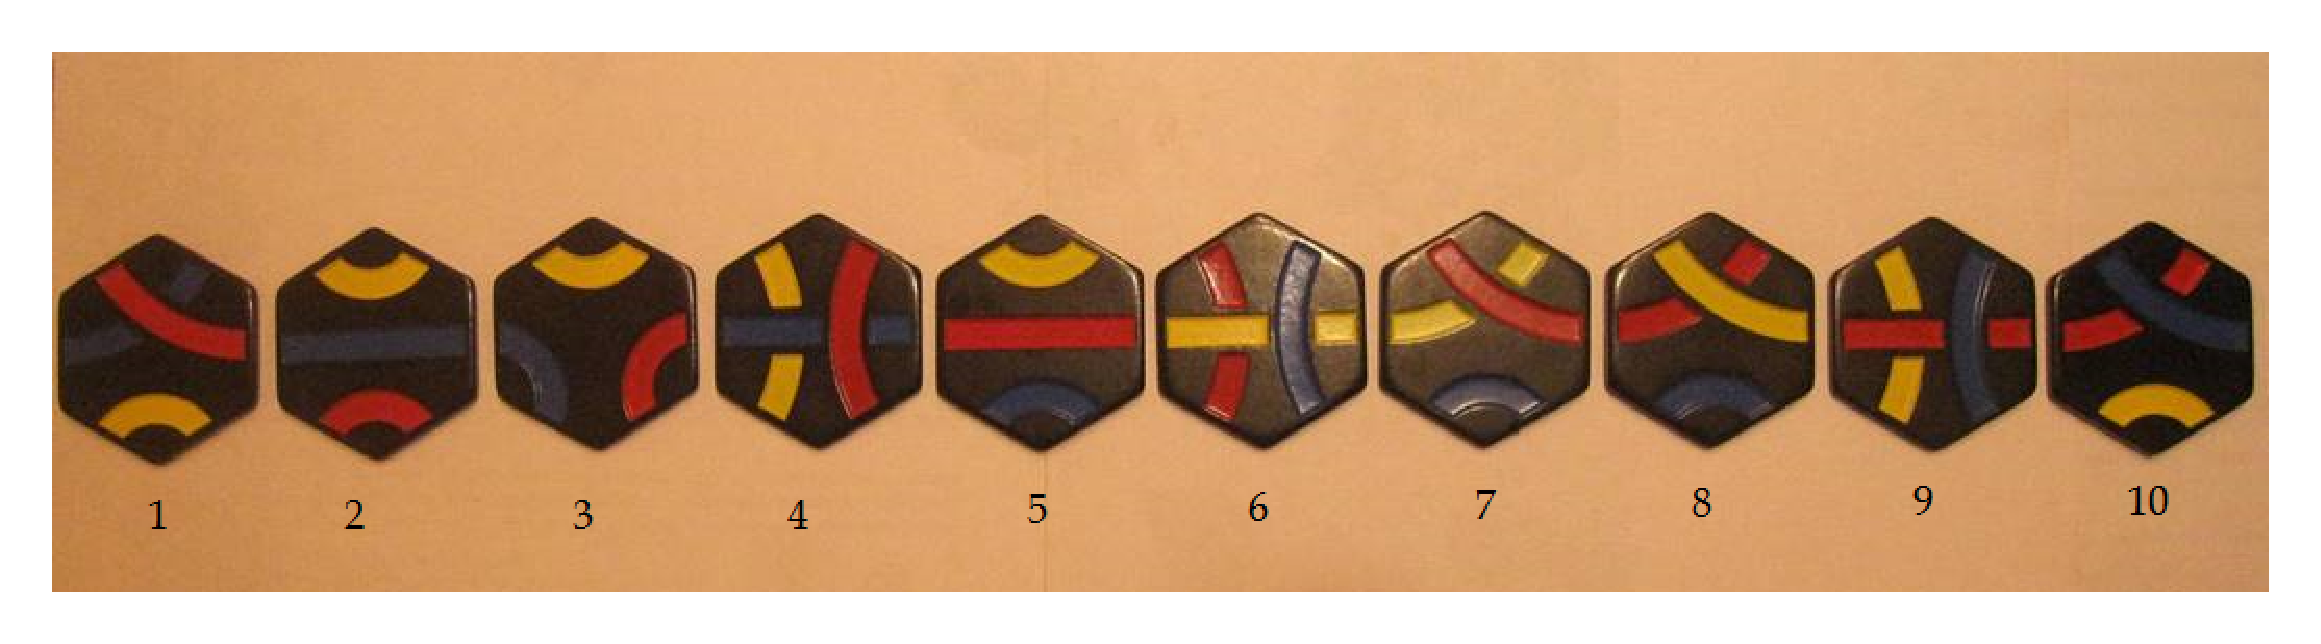
\includegraphics[width=1\linewidth]{Dozen_0.pdf}
        	\label{fig:mpr_-1}
        	\vspace{-25pt}
        	\caption{}
\end{figure}


\section{Описание данных}
Даннае представляют из себя изображения с фишками формата BMP. 
Каждая фишка представляет собой правильный шестиугольник черного цвета, на котором изображены сегменты трёх линий синего, красного и жёлтого цветов. Каждая линия имеет определенный тип: короткая дуга малой кривизны, длинная дуга большой кривизны или прямолинейный сектор.
Изображения  могу содержать либо одну фишку (рис. 2), либо группы из нескольких фишек (рис. 3).

\begin{figure}[H]
\centering
\begin{minipage}{.5\textwidth}
  \centering
  \includegraphics[width=0.8\linewidth]{Single_3.jpg}
  \label{fig:mpr_0}
  \vspace{0pt}
   \caption{}
\end{minipage}%
\begin{minipage}{.5\textwidth}
  \centering
   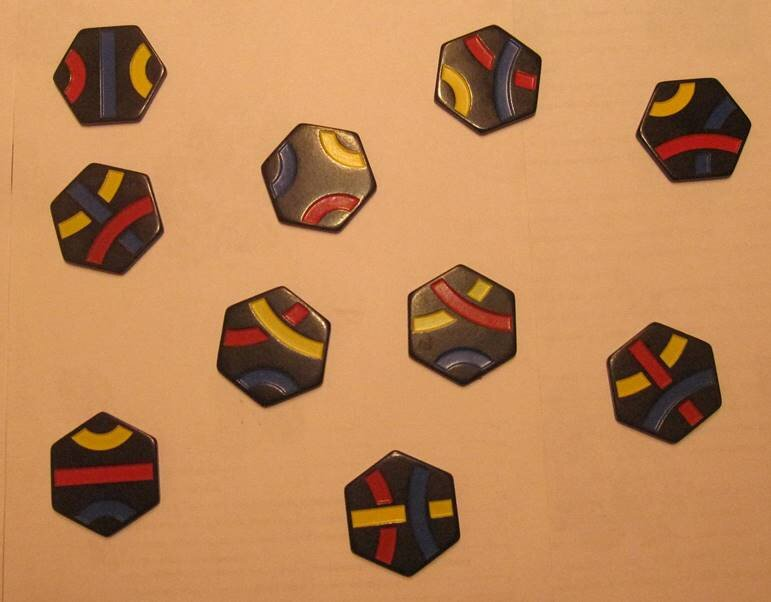
\includegraphics[width=0.9\linewidth]{Group_5.jpg}
   \label{fig:mpr_1}
   \vspace{0pt}
   \caption{}
\end{minipage}
\end{figure}


\section{Метод решения}  

Для решения задачи применяется следующий алгоритм: 


\begin{enumerate}
        \item Находятся контуры и периметры всех фишек, затем делается апроксимация полученных контуров для вычисления координат 6 углов каждой фишки
        \item Если на изображении несколько фишек, то каждая из них вырезается  по контурам, полученным в пункте 1. Затем для полученных картинок применяется путкт 1. 
        \item Находятся центры граней фишки с помощью координат углов, вычисленных выше.
        \item Находятся маски каждой дуги по ее цвету, диапазон цветов подбирался вручную.
        \item Создаются специальные маски для каждой грани фишки: на черном фоне рисуется белый круг с центром в середине грани и радиусом равным половине длины стороны грани. 
        \item Премножаются каждая из 6 маскок, полученных на шаге 5(маски с кругом в центре грани) с каждой из 3 масок, полученных на шаге 4(маски цвета) и вычисляется число белых пикселей. В итоге для каждой грани получается количество пикселей каждого цвета в ее окрестности. Идея состоит в том, что вблизи каждой грани больше цвета той дуги, которая к ней примыкает. Таким образом приписываем каждой гране цвет, количество пикселей которого больше. 
        В идеальном варианте должно получиться, что каждому цвету соответствует две грани. 
        \item На шаге 6 для каждого цвета полученны два номера грани. По эти номерам вычисляется вид дуг:
        \begin{itemize}
            \item Для каждого цвета находится модуль разности сторон (обозначим r)
            \item Если r > 3, то r = 6 - r
            \item Затем классифицируется вид дуги по найденному r:
                \begin{itemize} 
                    \item r = 1 - короткая дуга малой кривизны
                    \item r = 2 - длинная дуга большой кривизны
                    \item r = 3 - прямолинейный сектор
                \end{itemize}
        \end{itemize}
        \item Тип и цвет дуг позволяет однозначно определить номер почти всех фишке. Исключение составляют номера 7-8 и 1-10. Для различия этих типов учитывается следующая особеннность: при поиске контуров нумерация граней фишки происходит по часовой стрелке(нумерация с 0). На типе фишек 7-8 синяя дуга имеет малую кривизну, следовательно разность номеров ее граней равна 1, либо грани имеют номера 0 и 5. Найдем максимальный номер i среди номеров синих граней, а если номера 0 и 5, то берем 0. Затем смотрим цвет грани i+1. Если цвет  желтый, то тип - 7, иначе 8. Аналогичные действия проводятся для  определения типов 1 и 10.        
\end{enumerate}

\section{Описание программой реализации}

Программная реализация находится в файле task\_1.ipynb. Для работы с изображениями используется библиотека open\_cv.

Для удобства использования программы написанны функции 

\textbf{read\_image(path)} - чтение изображения с именем path, 

\textbf{show\_image(image)} - вывод изображения на экран, 

\textbf{draw\_contours(image, contours)} - возвращает изображение с нарисованными контурами. 

Для нахождения контуров на изображении написана функция 
\textbf{find\_contours(image)} - возвращает массив контуров на изображении. Она преобразует изображение к черно-белому и находит контуры с помощью функции  \textbf{cv2.findContours}

Для нахождения углов и периметров фишек реализованна 

функция  \textbf{find\_angles\_and\_per
(contours, eps)}, которая аппроксимирует найденные контуры с заданной точностью с помощью функции \textbf{cv2.approxPolyDP} и находит периметры контуров. Далее среди всех контуров с помощью периметров выделяются контуры фишек. Алгоритм основан на идее, что периметры всех фишек отличаются не сильно, и других фигур с похожим периметром на изображении нет. 


Результат работы функций представлен на картинке: 

\begin{figure}[H]
        	\centering
        	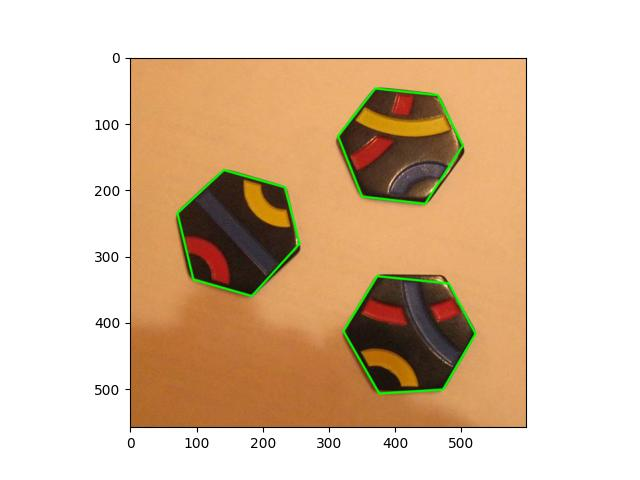
\includegraphics[width=0.7\linewidth]{contours_1.jpg}
        	\label{fig:mpr_2}
        	\vspace{-25pt}
        	\caption{}
\end{figure}

С помощью данных функций легко можно вычислить количество фишек на изображении, как количество найденных контуров. Для этого написана дополнительная функция \textbf{count\_chips(image)}, возвращающая одно число - количество фишек на изображении.


Далее реализованна функция \textbf{color\_mask(image, h\_min, h\_max)} которая по заданному изображению строит маску для цветов, попадающий в диапазон  [h\_min, h\_max]. Для этого изображение приводится к типу hsv, где первая компонента h отвечает за цвет. Далее с помощью функции \textbf{cv2.inRange} получается нужная маска. 

Результат работы функций представлен на картинке: 

\begin{figure}[H]
        	\centering
        	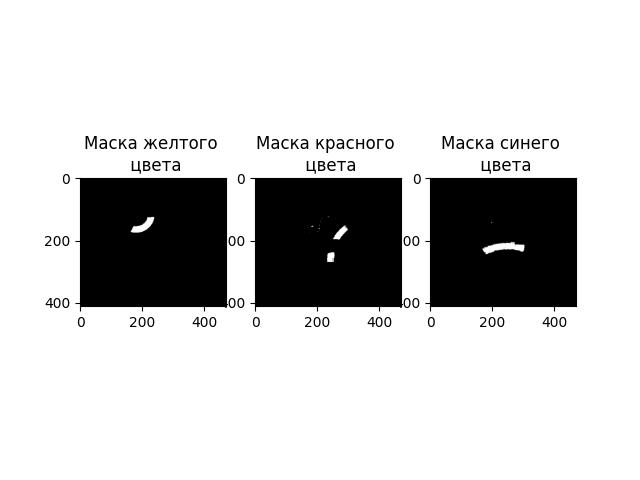
\includegraphics[width=0.5\linewidth]{mask_y.jpg}
        	\label{fig:mpr_3}
        	\vspace{-25pt}
        	\caption{}
\end{figure}


Одна из главных функций - \textbf{color\_and\_size(image)} - определяет цвета и типы дуг на изображениях с одной фишкой. С помощью описанных выше функций она находит углы фишки, (если их оказывается больше 6, то находятся ближайшие пары углов и оставляется один из них), вычисляет центры каждой из 6 граней, строит маски цвета. Затем по алгоритму, описанному выше(пункты 6 и 7 алгоритма) вычисляются номера сторон для каждого цвета.

С помощью этой функции написанна функция \textbf{print\_color\_and\_size(image)}, которая печатает результаты работы функции \textbf{color\_and\_size(image)} в более удобном для пользавателя виде.
 Например, для картинки ниже функция выводит ответ : "Желтая дуга малой кривизны, красная дуга большой кривизны, синяя дуга большой кривизны"

 \begin{figure}[H]
        	\centering
        	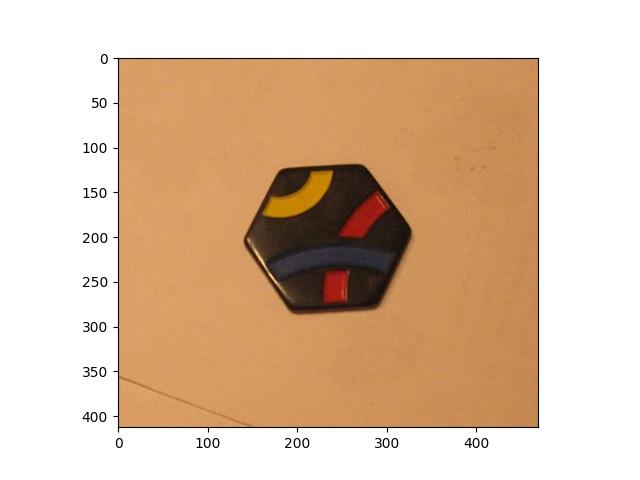
\includegraphics[width=0.5\linewidth]{Single_1.jpg}
        	\label{fig:mpr_4}
        	\vspace{-25pt}
        	\caption{}
\end{figure}

Основная функция для распознования типа фишек - \textbf{types\_chips(image)}. Она находит контуры фишек на изображении, вырезает каждую фишку по контуру и с помощью функции \textbf{color\_and\_size(image)} определяет типы дуг и номера фишек. Наконец, с помощью функции \textbf{cv2.putText} пишет номера фишек на изображении и возвращает его. 



\section{Эксперименты}  
Протестируем наш алгоритм. Для изображений с одной фишкой полученны следующие результаты:

 \begin{figure}[H]
        	\centering
        	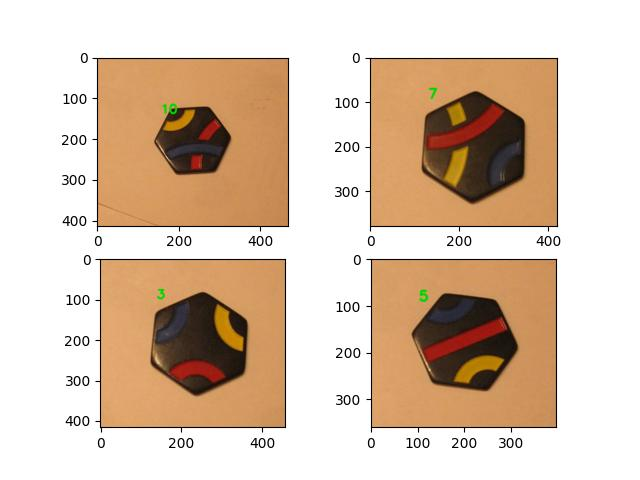
\includegraphics[width=1\linewidth]{test_1.jpg}
        	\label{fig:mpr_5}
        	\vspace{-25pt}
        	\caption{}
\end{figure}

Для групп фишек полученны следующие результаты:

 \begin{figure}[H]
        	\centering
        	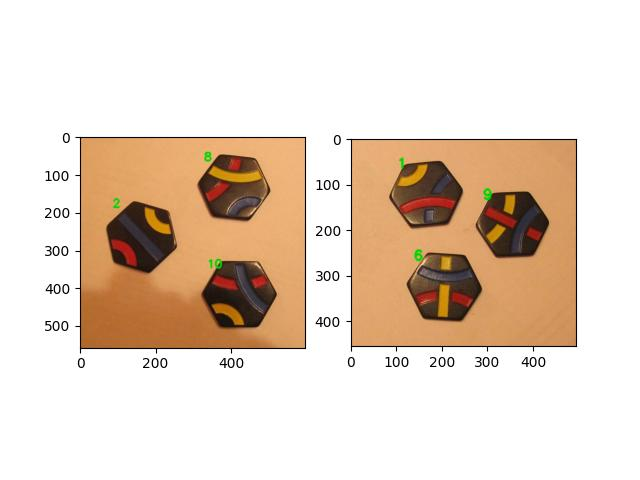
\includegraphics[width=0.8\linewidth]{test_3.jpg}
        	\label{fig:mpr_6}
        	\vspace{-25pt}
        	\caption{}
\end{figure}

 \begin{figure}[H]
        	\centering
        	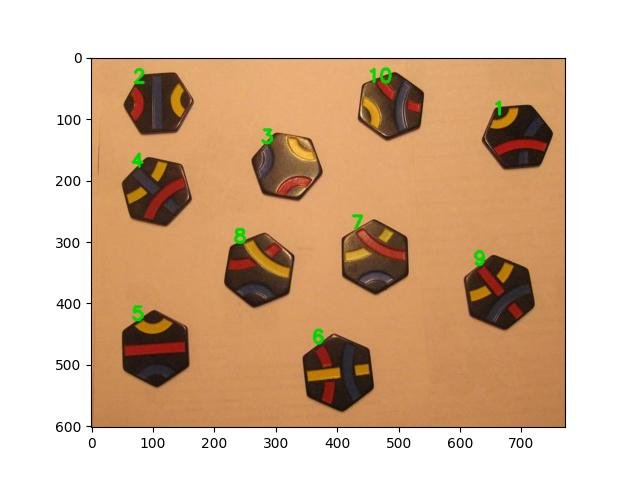
\includegraphics[width=1\linewidth]{test_2.jpg}
        	\label{fig:mpr_7}
        	\vspace{-25pt}
        	\caption{}
\end{figure}

Видим, что алгоритм правильно классифицирует фишки для данного набора картинок.


\section{Вывод}
    Была реализована программа, определяющая положение фишек и классифицирующая их в соответствии с заданными номерами.  Также, как вспомогательные задачи, были реализованы программы подсчета числа фишек на изображении и описания признаковых характеристик фишек - цвета и типа дуг. Алгоритм показал корректную работу на имеющихся данных.
\end{document}